\documentclass[main.tex]{subfiles}
\begin{document}

\marginpar{Tuesday\\ 2020-12-1, \\ compiled \\ \today}

We defined the neutron-to-proton ratio \(R_{np} = n_n / n_p\), and found 
%
\begin{align}
R_{np} = x_n^3 \qty[\frac{4 (1 + x_n^2)}{x_n^4 + 4 Q x_n^2 / m_n + 4 (Q^2- m_e^2) / m_n^2}]^{3/2}
\,.
\end{align}

In the \(x_n \gg 1\) limit, this is roughly a constant: \(R_{np} \sim 4^{3/2} = 8\).

\begin{figure}[ht]
\centering
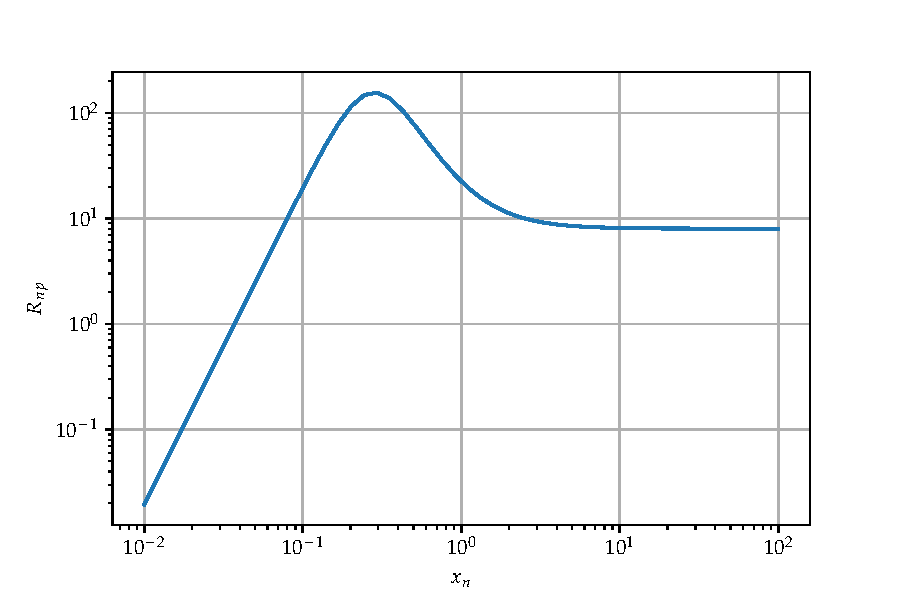
\includegraphics[width=\textwidth]{figures/neutron-proton-ratio}
\caption{Neutron-proton ratio as a function of \(x_n\).}
\label{fig:neutron-proton-ratio}
\end{figure}

\begin{figure}[ht]
\centering
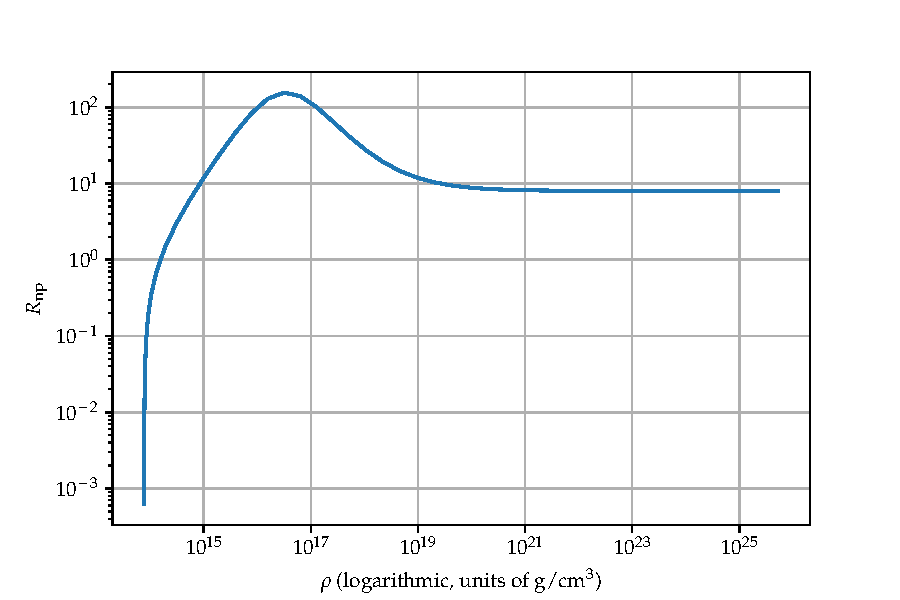
\includegraphics[width=\textwidth]{figures/neutron-proton-ratio-density}
\caption{Neutron-proton ratio as a function of the density \(\rho \) --- note the asymptote at \(\rho \sim \SI{e12}{g/cm^3}\), the lowest possible attainable density with neutrons, protons and electrons in equilibrium.}
\label{fig:neutron-proton-ratio-density}
\end{figure}

% For heavy nuclei we have the process:

% Above a certain density we start having neutron ``drip'' from heavy nuclei.
\todo[inline]{Add part about internal structure?}

\begin{figure}[]
\centering
\includegraphics[width=\textwidth]{figures/NS-interior}
\caption{Stolen image.}
\label{fig:NS-interior}
\end{figure}

\subsection{The URCA and MURCA processes}

The NS typically forms in a Core-Collapse Supernova event, thus starting with temperatures of the order of \SI{e11}{K}, and then cools (we know this since the NSs we have observed are typically much colder than that). Let us explore how this cooling happens.

At \(T > \SI{e10}{K}\), we will have to account for both photon and neutrino luminosity (\(L_\gamma \) and \(L_\nu \) respectively), as well as heating (\(H\)): the change in internal (thermal) energy will look like
%
\begin{align}
\dv{E _{\text{th}}}{t} = H - L_\gamma - L_\nu 
\,.
\end{align}

We also know that a change in energy can be related to a change in temperature in terms of the heat capacity \(c_V\),
%
\begin{align}
\dv{E _{\text{th}}}{t} = c_V \dv{T }{t}
\,,
\end{align}
%
therefore the differential equation for the temperature reads
%
\begin{align}
c_V \dv{T }{t} = H - L_\nu - L_\gamma 
\,.
\end{align}

We have the two processes of neutron decay and neutron formation (electron capture): let us write them in a rather generic form, in terms of a lepton \(\ell\) (typically an electron, but it could also be a muon), its corresponding neutrino \(\nu _\ell\), and a nuclide \((Z, A)\), where \(Z\) is the proton count while \(A\) is the total mass number (protons plus neutrons):
%
\begin{align}
(Z, A) + \ell \to (Z-1, A) + \nu_\ell
&&
(Z, A) \to (Z+1, A) + \ell + \overline{\nu}_\ell
\,.
\end{align}

These constitute the direct URCA process. 
URCA was a famous Casino in Rio in the fifties, and the name was proposed by George Gamow, who liked gambling: 
the idea is that if these two processes were to occur at equilibrium then energy would be lost by a NS ``as fast as money is lost at URCA'' --- this is known as a ``fast'' neutrino-producing process.

We will see why, but first let us calculate a \textbf{condition for the URCA process to occur}.
By momentum conservation, neglecting the momentum of the neutrino,\footnote{It is indeed negligible since this is all happening in a degenerate gas of neutrons, protons and electrons: therefore, their momenta must be very high since the low-momentum states are saturated; on the other hands neutrinos quickly escape, so their number density is very low, they are not degenerate.} we will have \(\vec{p}_n = \vec{p}_p + \vec{p}_e\); however all three species are degenerate, therefore this equality must also hold for the Fermi momenta. 

By the triangle inequality we know that \(p_{Fn} \leq p_{Fp} + p_{Fe}\), and by charge neutrality we also know that \(n_e = n_p\), therefore  \(p_{Fe} = p_{Fp}\), therefore \(p_{Fn} \leq 2 p_{Fp}\). 

Finally, this yields \(n_n \leq 8 n_p\), or \(R_{np} \leq 8\). Therefore, 
%
\begin{align}
\frac{n_p}{n_n + n_p} \geq \frac{1}{9}
\,.
\end{align}

% This contradicts what we found for \(R_{np}\): we learned that. 
As we have seen when we have calculated \(R_{np} (x_n)\), this can be achieved for very small densities, so \(x_n \lesssim \num{.1}\), or in the limit of very large \(x_n\).
Qualitatively speaking, if the density is too large there is \textbf{Pauli blocking} of the reaction --- the momentum ``spots'' in which the products would land are already filled. 

So, we need a process to allow for cooling in the higher-density case.
We could have exotic particles like hyperons or kaons; however there is no direct evidence for them, so first we should look to second order processes, which include a bystander, like
%
\begin{align}
\ce{n} + \ce{n} \to e^{-} + \ce{p} + \overline{\nu} + \ce{n}
\,,
\end{align}
%
which is called the \(n\)-channel, and similarly we have the \(p\)-channel, in which the bystander is a proton. 
This is the Modified URCA process, or MURCA. This is slow. 

The neutrino emissivities can be shown to look like
%
\begin{align}
\epsilon _\nu^{\text{URCA}} &\approx \num{e27} R(\rho, T) \qty(\frac{T}{\SI{e9}{K}})^{6} \SI{}{erg cm^{-3} s^{-1}} \\
\epsilon _\nu^{\text{MURCA}} &\approx \num{e21} R(\rho, T) \qty(\frac{T}{\SI{e9}{K}})^{8} \SI{}{erg cm^{-3} s^{-1}}
\,,
\end{align}
%
where \(R\) is a slowly-changing function of \(\rho \) and \(T\); the total neutrino luminosity (at constant temperature) is found by integrating the emissivities over the volume,
%
\begin{align}
L_\nu = \int \epsilon _\nu \dd{V}
\,.
\end{align}

With this, we find that the neutrino luminosity for slow processes (MURCA) is \(L_\nu^{s} = N^{s} T^{8}\), while \(L_\nu^{f} = N^{f} T^{6}\), where \(N^{s}\) and \(N^{f}\) are two constants (with dimensions) whose approximate expressions are given before. 

\begin{figure}[H]
\centering
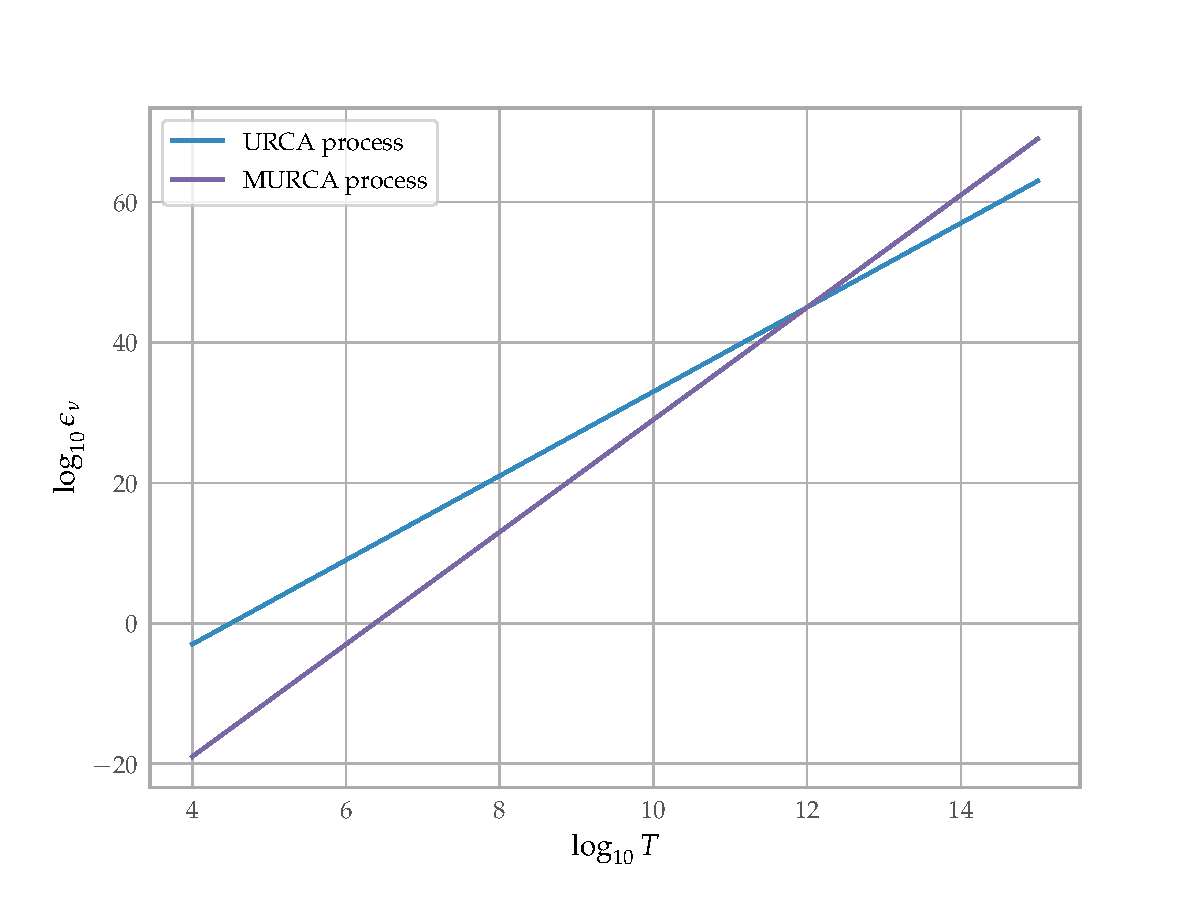
\includegraphics[width=.7\textwidth]{figures/urca-murca}
\caption{URCA and MURCA emissivities.}
\label{fig:urca-murca}
\end{figure}

On the other hand, the photon luminosity can be approximated through blackbody radiation: 
%
\begin{align}
L_\gamma = 4 \pi R^2 \sigma T_e^4
\,,
\end{align}
%
where \(T_e\) is the surface temperature, and it is different from \(T\) (typically much lower than it). 
This is due to the presence of an envelope around the neutron star, which emits the bulk of the radiation. 

Typically, we can take \(T = \const\) inside the core, and \(T_e \propto T^{1/2 + \alpha }\), with \(\alpha \ll 1\), so \(T_e \sim \sqrt{T}\).

This then tells us that \(L_\gamma = S T^{2 + 4 \alpha }\). 
Also, we can say that for a degenerate system \(c_V \approx c T\) for some constant \(c\).\footnote{The heat capacity is defined as the derivative of the internal energy with respect to temperature. For a classical gas it would be \(c_V \propto N k_B\) with some constant accounting for the degrees of freedom; for a degenerate gas it is much lower since increasing the temperature only shifts the ``edge'' of the distribution, near the Fermi energy. 

The full calculation may be done or approximated, but let us give a qualitative argument. As the temperature increases from \(T = 0\), a fraction of the electrons of the order \(k_B T / E_F\) gets its temperature increased by \(k_B T\). Therefore, \(\Delta U \propto T^2\), which means that \(c_V \propto T\). In the classical case, on the other hand, \emph{all} the gas particles get their energies increased, meaning that \(\Delta U \propto T\), so \(c_V \propto T^{0}\).}
Substituting this in, the cooling law reads 
%
\begin{align}
c T \dv{T}{t} = - L_\nu - L_\gamma 
\,,
\end{align}
%
and as we will see \(L_\nu \gg  L_\gamma \), therefore if MURCA dominates over URCA and photons we have 
%
\begin{align}
cT \dv{T}{t} = - N^{s} T^{8}
\,,
\end{align}
%
which yields 
%
\begin{align}
\frac{ \dd{T}}{T^{7}} &= - \frac{N^{s}}{c} \dd{t}  \\
\frac{1}{6} \qty( \frac{1}{T^{6}} - \frac{1}{T _{\text{in}}^{6}}) &= \frac{N^{s}}{c} (t - t _{\text{in}})
\,.
\end{align}

If \(T _{\text{in}} \gg T\) (which is realistic with SN formation scenarios) we will have 
%
\begin{align}
\frac{c}{6 N^{s}} t^{-1} = T^{6} \implies T \propto t^{-1/6}
\,.
\end{align}

We can make a very similar calculation for the URCA process: this yields  \(T \propto t^{-1/4}\), a steeper decrease. 

The fast process timescale looks like 
%
\begin{align}
\tau^f_\nu = \frac{c}{4 N^{f} T^{4}} = 4 \qty(\frac{c_{30}}{10 N^{s}_{\num{.62}} T^{4}_9}) \SI{}{s}
\,,
\end{align}
%
which is much shorter than the corresponding slow timescale 
%
\begin{align}
\tau^s_\nu = \frac{c}{6 N^{s} T^{6}}  = 6 \qty(\frac{c_{30}}{6 N_{30}^{s} T^{4}_9}) \SI{}{months}
\,.
\end{align}



\end{document}
